\documentclass[10pt]{article}
\usepackage[a4paper, margin=1in]{geometry}
\usepackage[utf8]{inputenc}
\usepackage[spanish]{babel}
\usepackage{caratula}
\usepackage{amsmath}
\usepackage{amssymb}
\usepackage{hyperref}
\usepackage{enumitem}
\usepackage{graphicx}
\usepackage{subcaption} % Para subfiguras

\hypersetup{
    colorlinks=true,
    linkcolor=blue,
    filecolor=magenta,      
    urlcolor=cyan,
    pdftitle={Overleaf Example},
    pdfpagemode=FullScreen,
	}
	
\setlength{\parskip}{1em}   % Espacio vertical entre párrafos

\begin{document}

	\titulo{TP2}

	\fecha{\today}

	\materia{Introducción a la Investigación Operativa y Optimización}

	\integrante{Laks, Joaquín}{425/22}{laksjoaquin@gmail.com}
	\integrante{Szabo, Jorge}{1683/21}{jorgecszabo@gmail.com}
	\integrante{Wilders Azara, Santiago}{350/19}{santiago199913@gmail.com}

	\maketitle

\section{Introducción}

En este trabajo práctico abordamos el problema de distribución de productos a clientes con metodologías distintas, variaciones del problema del viajante, incorporando repartidores a pie o en bicicleta y productos refrigerados. En particular para estas metodologías, se busca identificar qué clientes deben ser visitados directamente por el camión y cuáles pueden ser atendidos por repartidores a pie/bicicleta desde determinadas paradas del camión, respetando restricciones operativas como la distancia máxima de reparto o la entrega de productos refrigerados.

El objetivo principal es modelar, generar instancias y analizar los resultados obtenidos para las distintas metodologías comparando sus costos. Además, se analizarán los tiempos de cómputo requeridos utilizando diferentes alternativas algorítmicas mediante los parámetros que provee CPLEX.

A continuación, se describen las distintas metodologías de reparto consideradas y los modelos propuestos para representarlas.
\section{Modelos}


\subsection{Modelo para la metodología actual (TSP)}

La metodología actual consiste en que el camión visita a cada cliente y entrega sus pedidos, es decir, idéntica al problema del viajante clásico. Usamos el modelo de Miller, Tucker, y Zemlin para simularlo y como base para las otras metodologías.

\subsection{Modelo con repartidores (MR)}

Se desea evaluar una nueva metodología de distribución en la cual el camión realiza paradas en ciertos clientes, y desde esas paradas se pueden realizar entregas adicionales mediante repartidores a pie o en bicicleta, siempre que los clientes estén a una distancia menor o igual a $dist\_max$. Cada repartidor tiene un costo por cliente atendido, y esta restringido a una única entrega en caso de que sea un producto refrigerado.


Basado en el modelo anterior, agregamos variables para distinguir cuándo un cliente fue visitado por repartidor a bicicleta y cuándo fue visitado por el camión.

	\vspace{5mm}

	Dado un cliente $i$, definimos $D_i$ como el conjunto de clientes a una distancia menor a \texttt{dist\_max} de $i$.
	
	\begin{align*}
		x_{ij} &= 
		\begin{cases}
			1 & \text{si el camión se mueve desde el cliente $v_i$ al cliente $v_j$} \\
			0 & \text{en caso contrario}
		\end{cases} \\[1em]
		u_i &= \text{posición del cliente $i$ en el circuito del camión (irrelevante si no es visitado)} \\[1em]
		b_{ij} &= 
		\begin{cases}
			1 & \text{si se envió un repartidor desde $v_i$ hasta $v_j$} \\
			0 & \text{en caso contrario}
		\end{cases} \\[1em]
		r_i &=
		\begin{cases}
			1 & \text{si al cliente $v_i$ se le entrega un producto que necesita refrigeración} \\
			0 & \text{en caso contrario}
		\end{cases}
	\end{align*}
	
\vspace{5mm}

\clearpage

	Entonces con $n = cant\_clientes$, buscamos:

	\[
		\text{Min} \sum_{\substack{v_i, v_j \in V \\ i \neq j}} c_{ij} x_{ij} 
		+ costo\_repartidor\, b_{ij}
		\]

	s.a.

	\[
	\begin{array}{l l l}
		\sum_{j \neq i} x_{ji} + \sum_{j \neq i} b_{ji} = 1 & \forall v_i \in V & \text{\scriptsize (a toda ciudad se entra una vez, por camión o bicicleta)} \\
		\\
		\sum_{j \neq i} x_{ij} = \sum_{j\neq i} x_{ji} & \forall v_i \in V & \text{\scriptsize (si se entró en camión, se sale por camión)} \\
		\\
		M(1 - \sum_{j \neq i} b_{ji}) \geq \sum_{j \neq i} b_{ij} + \sum_{j \neq i} x_{ij} & \forall v_i \in V, M \geq |V| & \text{\scriptsize (si se entra en bicicleta, no se sale de ninguna forma)} \\
		\\
		\sum_{j \in D_i} b_{ij} r_j \leq 1 & \forall v_i \in V & \text{\scriptsize (ningún repartidor tiene más de un refrigerado)} \\
		\\
		u_i - u_j + (n - 1) x_{ij} \leq n - 2 & \forall v_i \neq v_j \in V - \{v_1\} & \text{\scriptsize (continuidad)} \\
		\\
		u_1 = 0, 1 \leq u_i \leq n-1 & \forall v_i \in V - \{v_1\} \\
		\\
		x_{ij}, b_{ij} \in \{0,1\}, u_i \in \mathbb{Z}_{\geq 0}
	\end{array}
	\]
	
	
	
	\subsection{Modelos con restricciones agregadas (MR4 y MRE)}
	
	Estos metodologías extienden la anterior incorporando una nueva restricción adicional en cada caso:
	
	\begin{description}
		\item[MR4:] Si se contrata un repartidor en una parada de camión determinada, este debe realizar al menos cuatro entregas.
		\item[MRE:] Hay un conjunto de clientes $E$ que deben ser visitados exclusivamente por un camión. Es decir, sus paquetes no pueden ser repartidos por un repartidor en bicicleta.
	\end{description}
	
	Entonces, para cada modelo se extiende el presentado en la sección anterior con su respectiva nueva restricción:
	
	\begin{description}
		\item[MR4:]
		\[
		4(1 - b_{ij}) + \sum_{v_k \in D_i} b_{ik} \geq 4 \quad \forall v_i, v_j \in V \times V
		\]
		
		\item[MRE:]
		\[
		\sum_{v_i \in V}  b_{ij} = 0 \quad \forall v_j \in E
		\]
	\end{description}
	
	No hay cambios en las variables, función objetivo o las demás restricciones.

\clearpage

\section{Comparación de costos entre metodologías}
Para analizar el rendimiento de las distintas metodologías, definimos y generamos dos tipos distintos de instancias, uno con clientes uniformemente distribuidos y el otro conformado por varios clusters distintos donde se concentran grupos de clientes dentro de un radio. En las figuras~\ref{fig:compuesta1} y~\ref{fig:compuesta2} respectivamente, se puede apreciar la diferencia de los tipos.

\vspace{5mm}

\begin{figure}[htbp]
	\centering
	\begin{subfigure}[b]{0.45\textwidth}
		\centering
		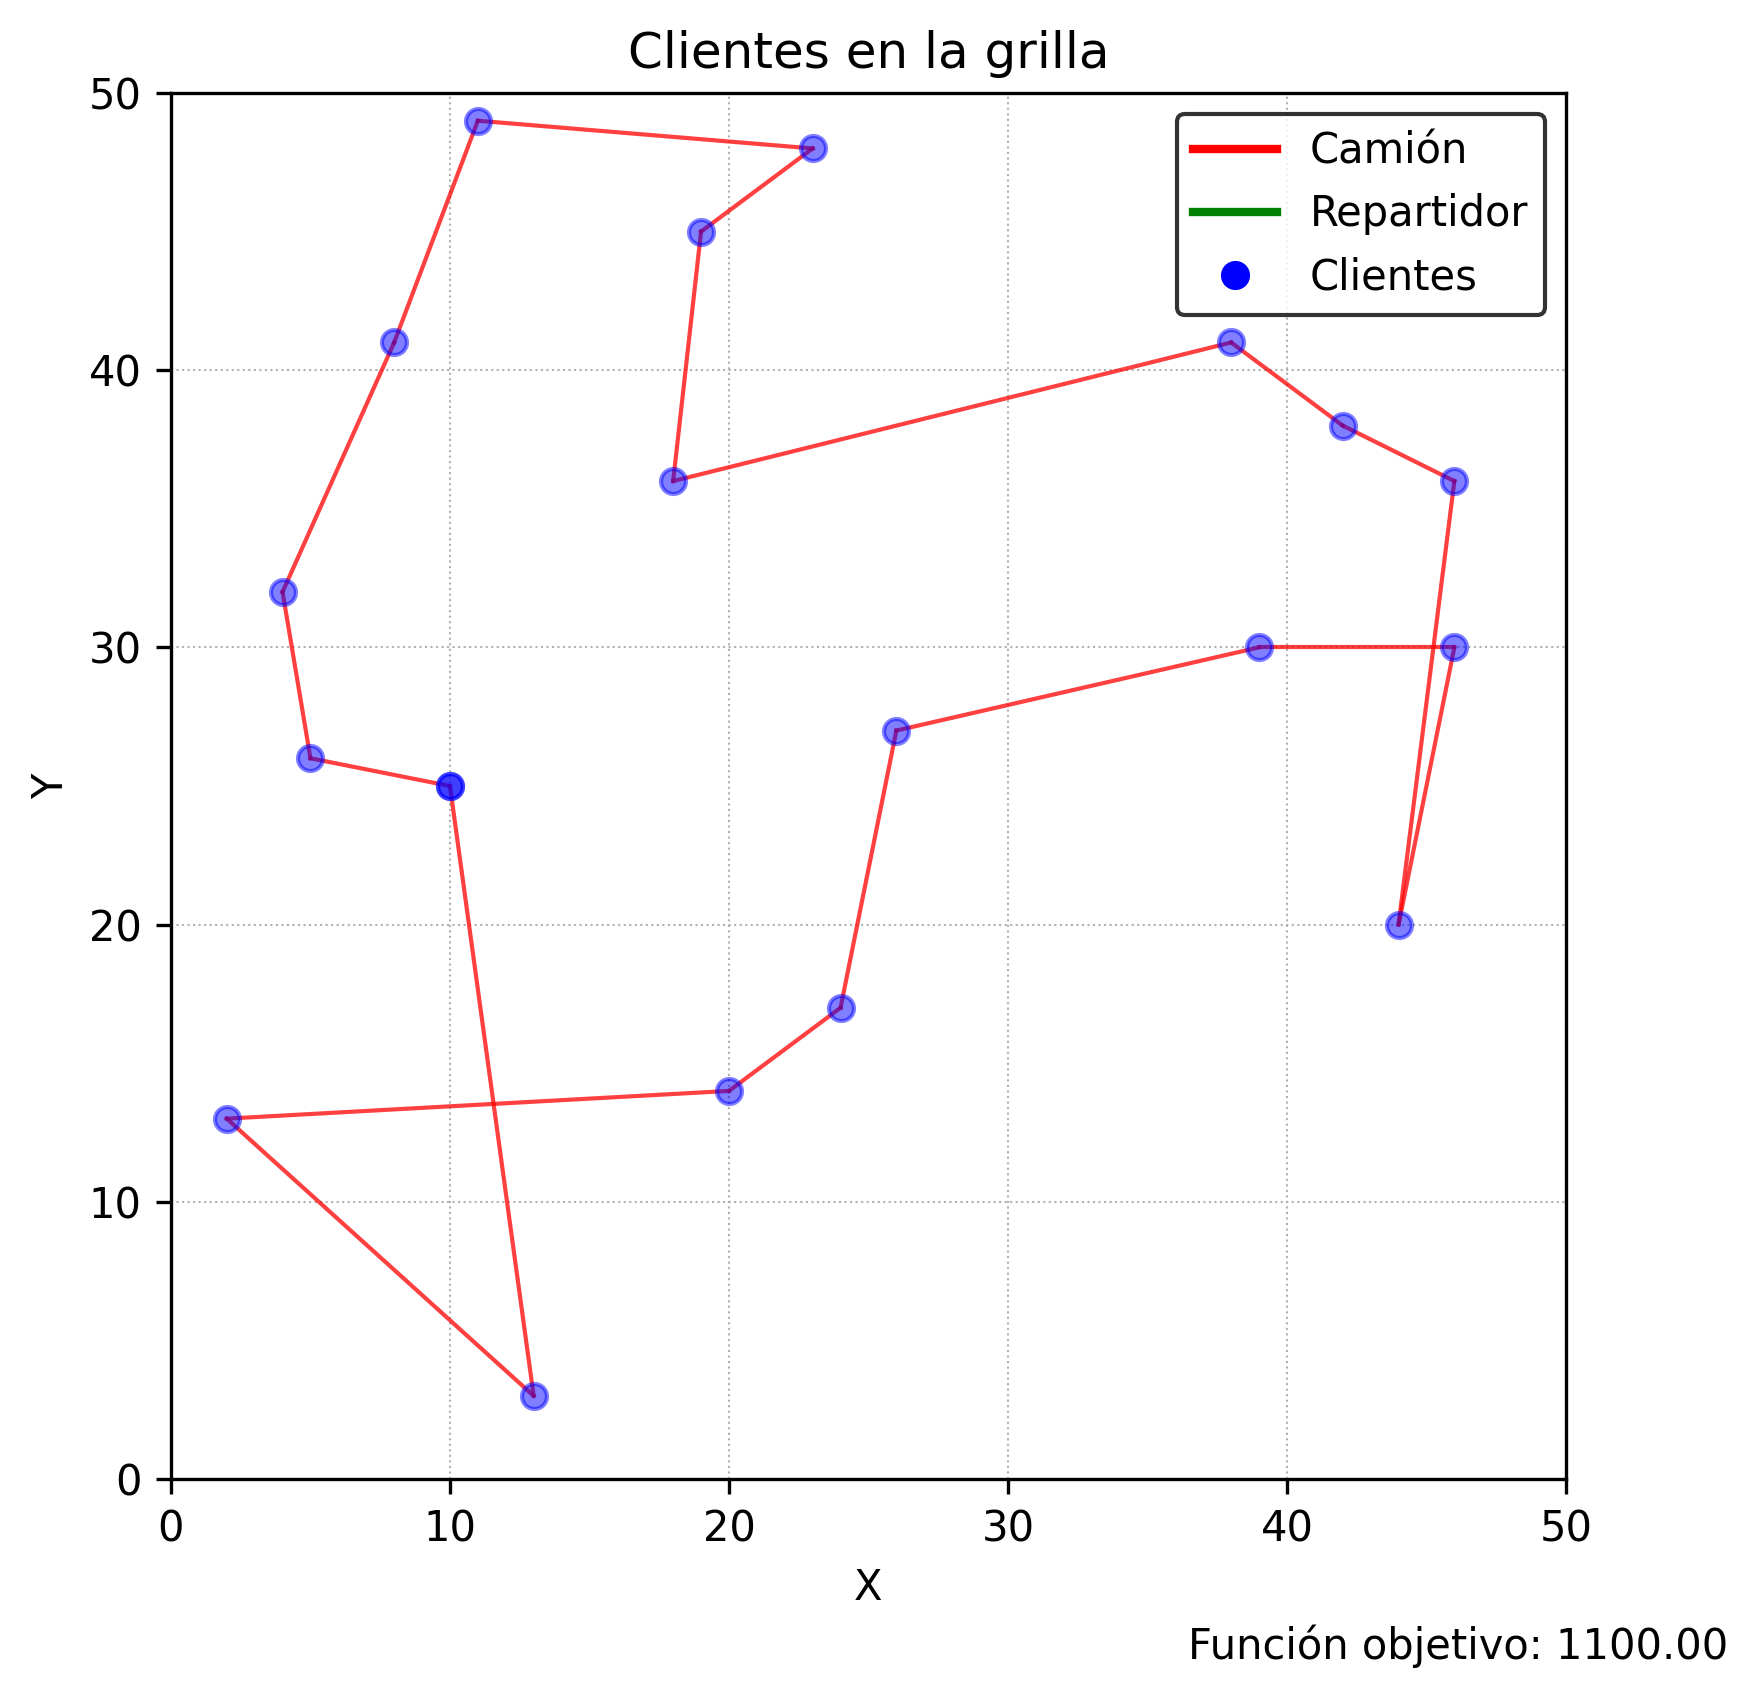
\includegraphics[width=\textwidth]{figuras/plano_uniforme_tsp_2.png}
		\caption{Metodología actual (TSP)}
		\label{fig:sub1}
	\end{subfigure}
	\hfill
	\begin{subfigure}[b]{0.45\textwidth}
		\centering
		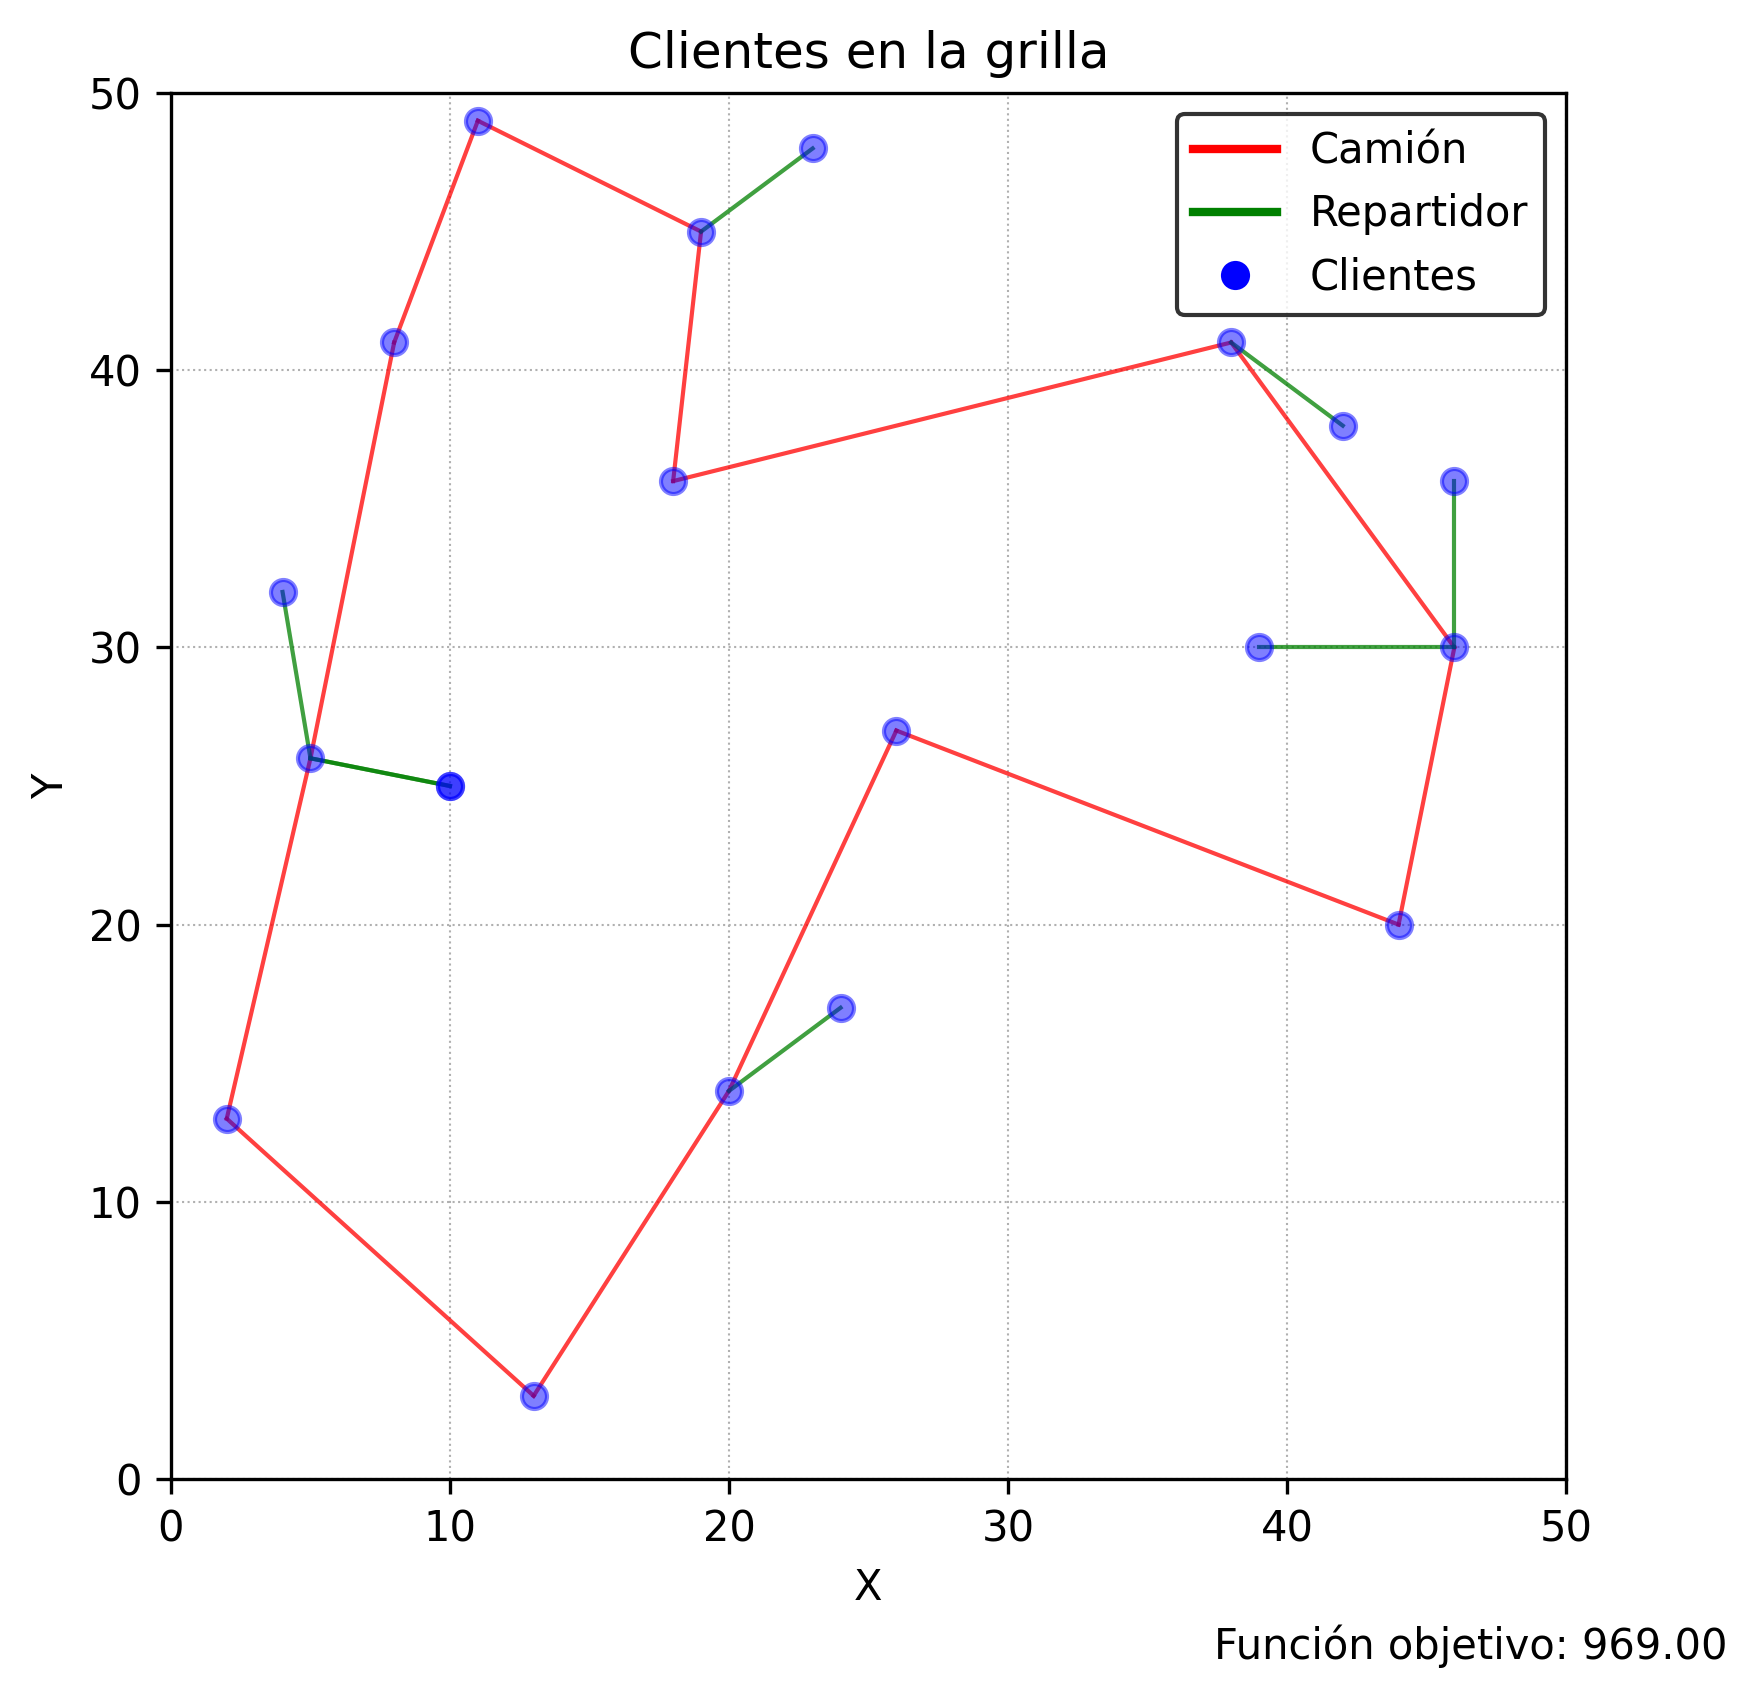
\includegraphics[width=\textwidth]{figuras/plano_uniforme_repartidores_2.png}
		\caption{Metodología con repartidores (MR)}
		\label{fig:sub2}
	\end{subfigure}
	
	\vspace{0.5cm}
	
	\begin{subfigure}[b]{0.45\textwidth}
		\centering
		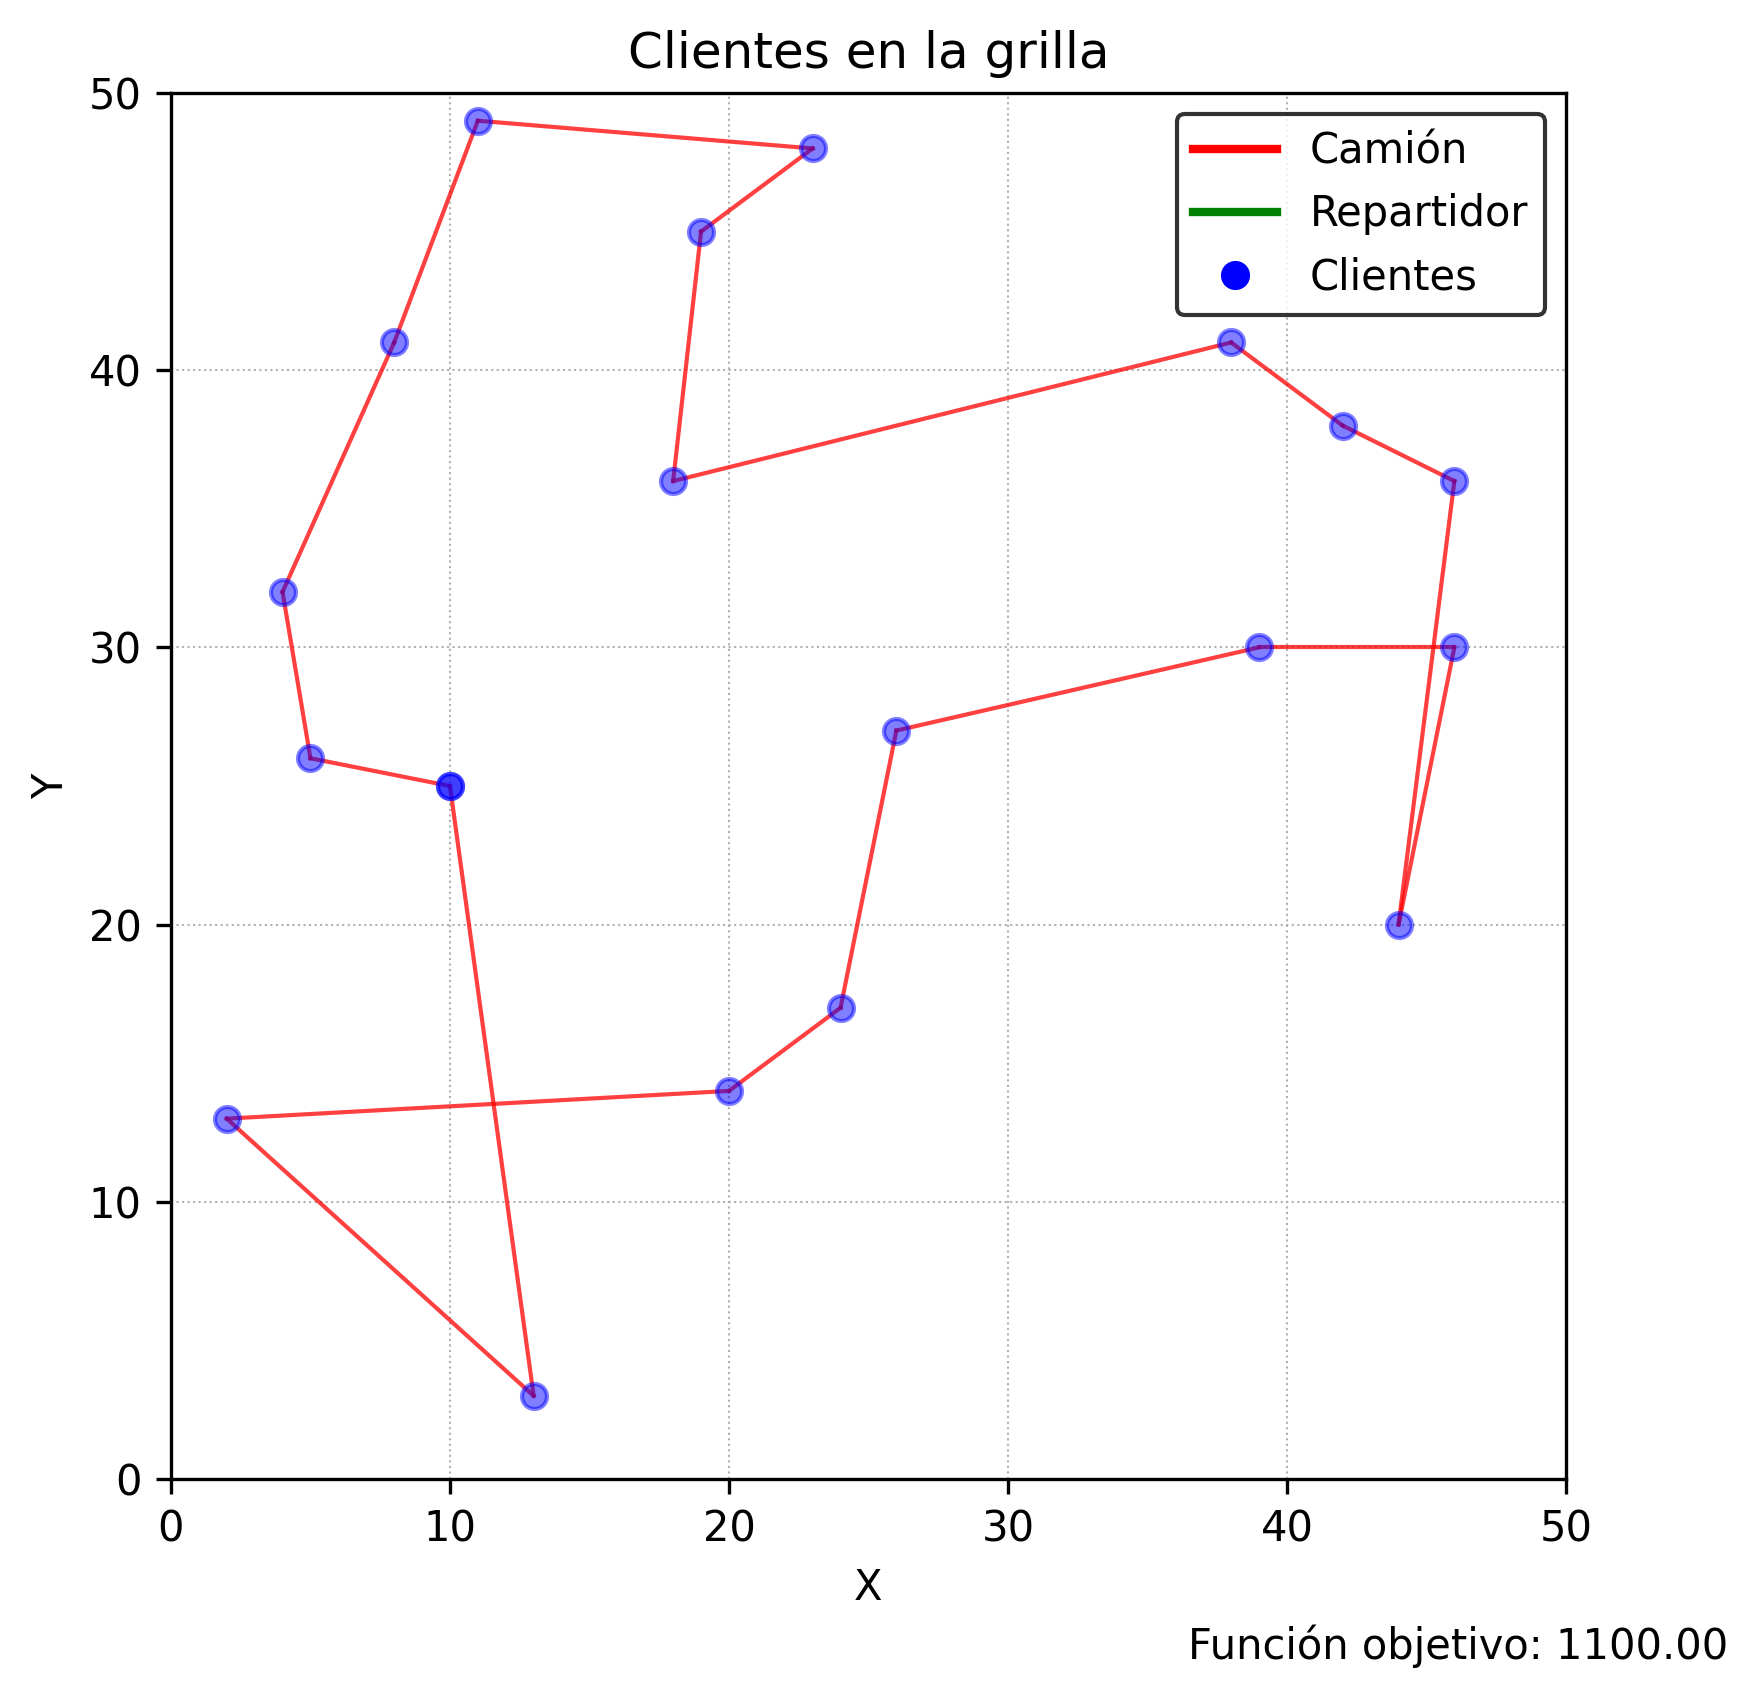
\includegraphics[width=\textwidth]{figuras/plano_uniforme_cuatro_o_mas_2.png}
		\caption{Metodología con repartidores de al menos cuatro entregas (MR4)}
		\label{fig:sub3}
	\end{subfigure}
	\hfill
	\begin{subfigure}[b]{0.45\textwidth}
		\centering
		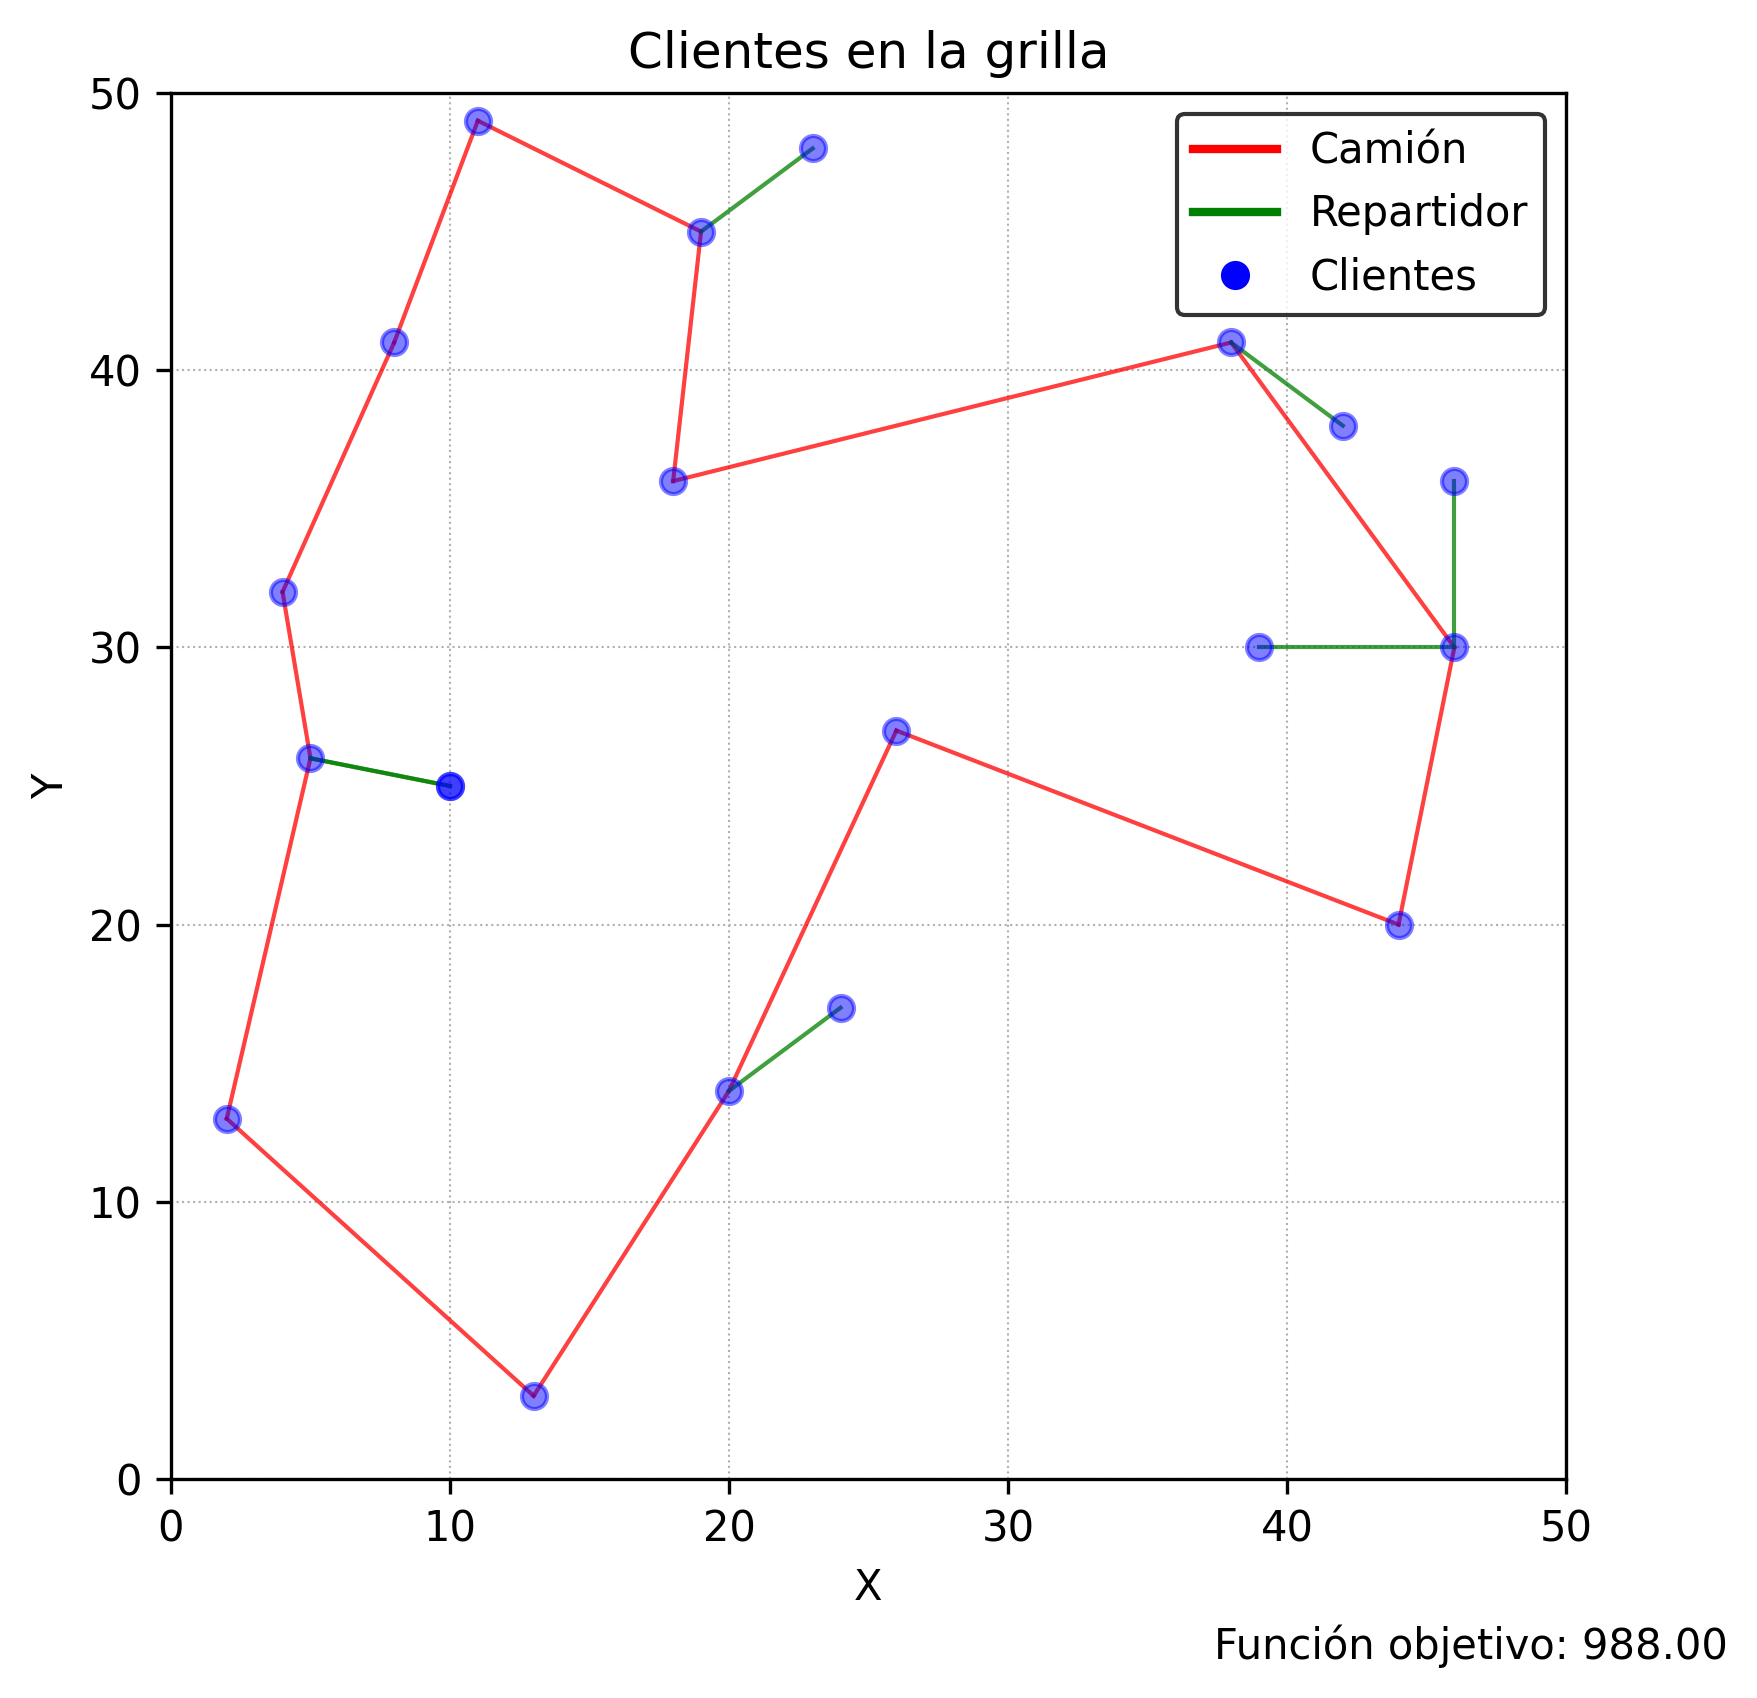
\includegraphics[width=\textwidth]{figuras/plano_uniforme_exclusivos_2.png}
		\caption{Metodología con clientes exclusivos (MRE)}
		\label{fig:sub4}
	\end{subfigure}
	
	\caption{Optimización de una misma instancia \textbf{uniformemente distribuida} con los distintos modelos.}
	\label{fig:compuesta1}
\end{figure}

\clearpage

\begin{figure}[htbp]
	\centering
	\begin{subfigure}[b]{0.45\textwidth}
		\centering
		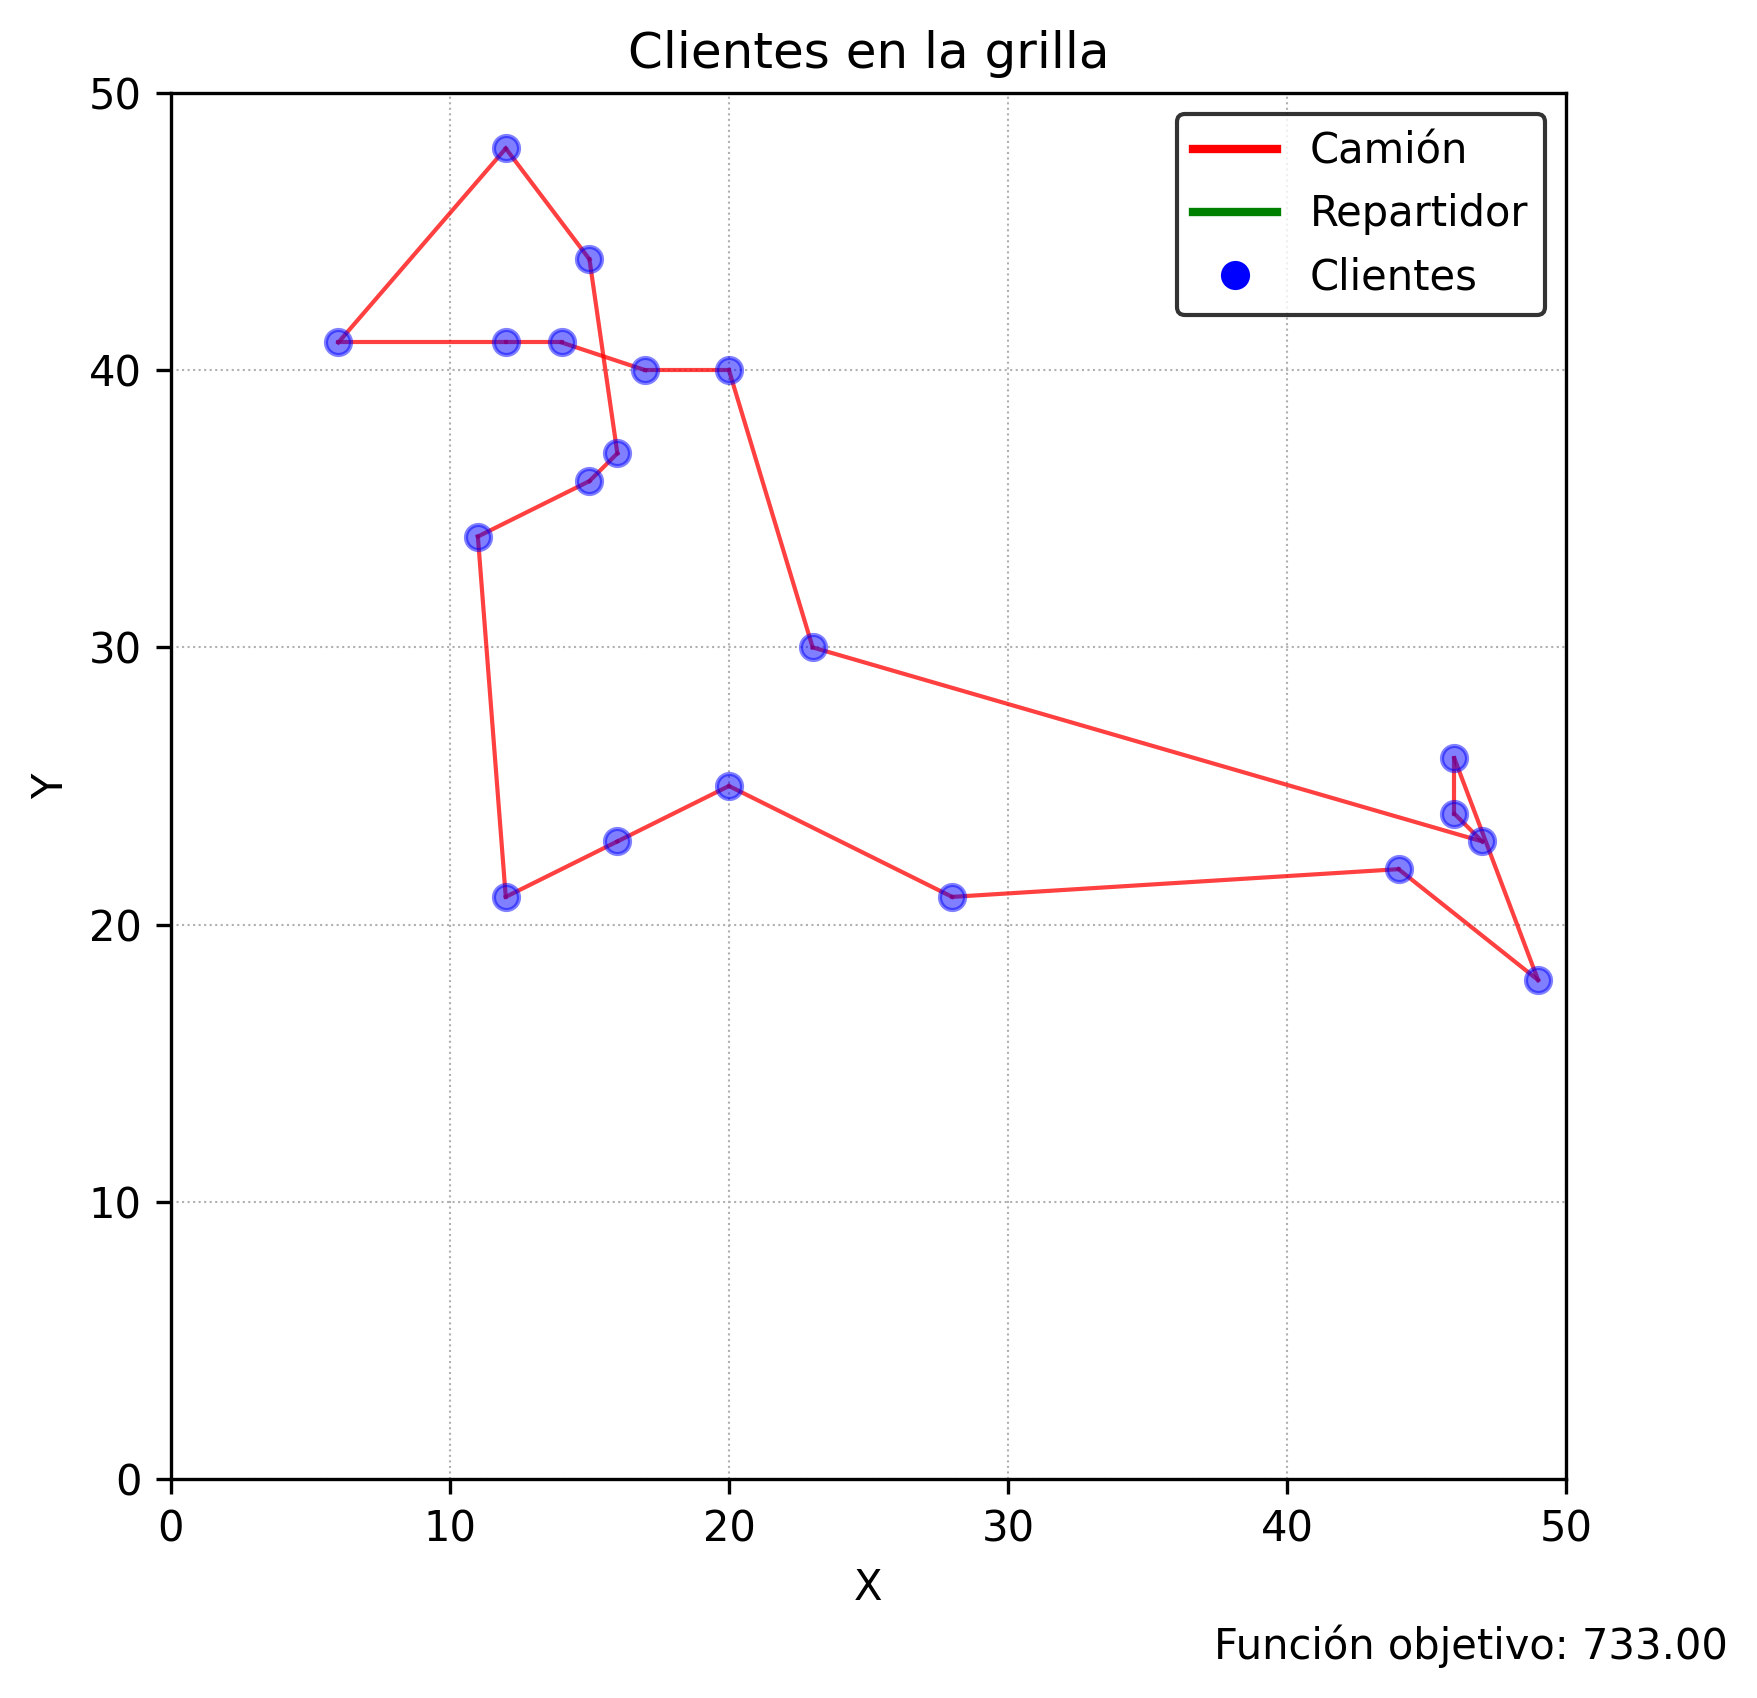
\includegraphics[width=\textwidth]{figuras/plano_clusters_tsp_0.png}
		\caption{Metodología actual (TSP)}
		\label{fig:sub1}
	\end{subfigure}
	\hfill
	\begin{subfigure}[b]{0.45\textwidth}
		\centering
		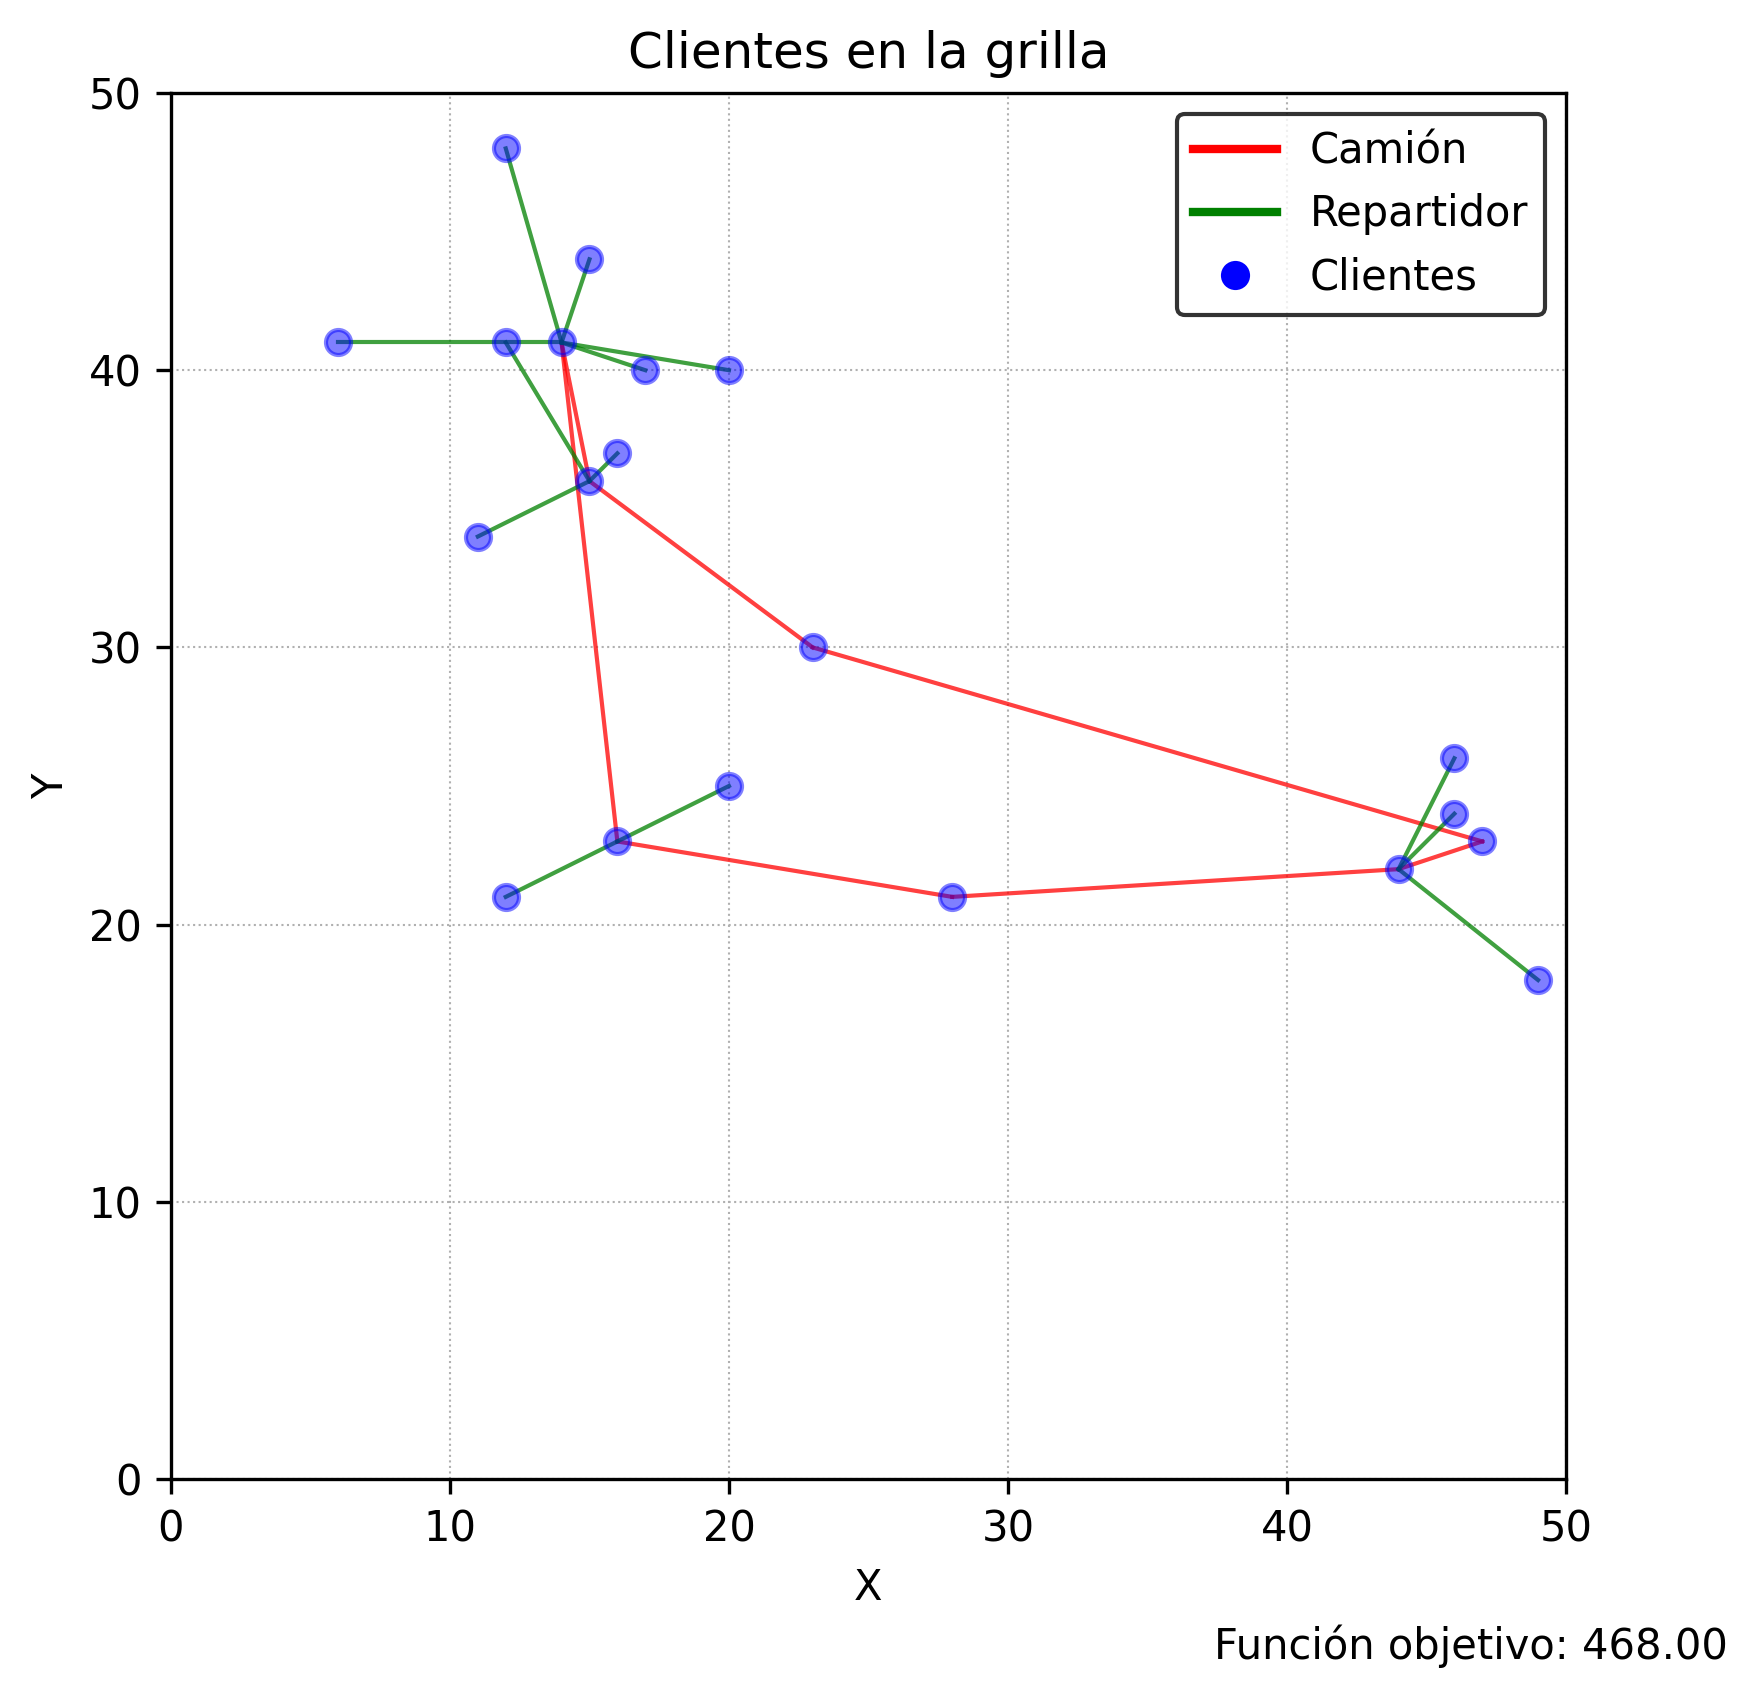
\includegraphics[width=\textwidth]{figuras/plano_clusters_repartidores_0.png}
		\caption{Metodología con repartidores (MR)}
		\label{fig:sub2}
	\end{subfigure}
	
	\vspace{0.5cm}
	
	\begin{subfigure}[b]{0.45\textwidth}
		\centering
		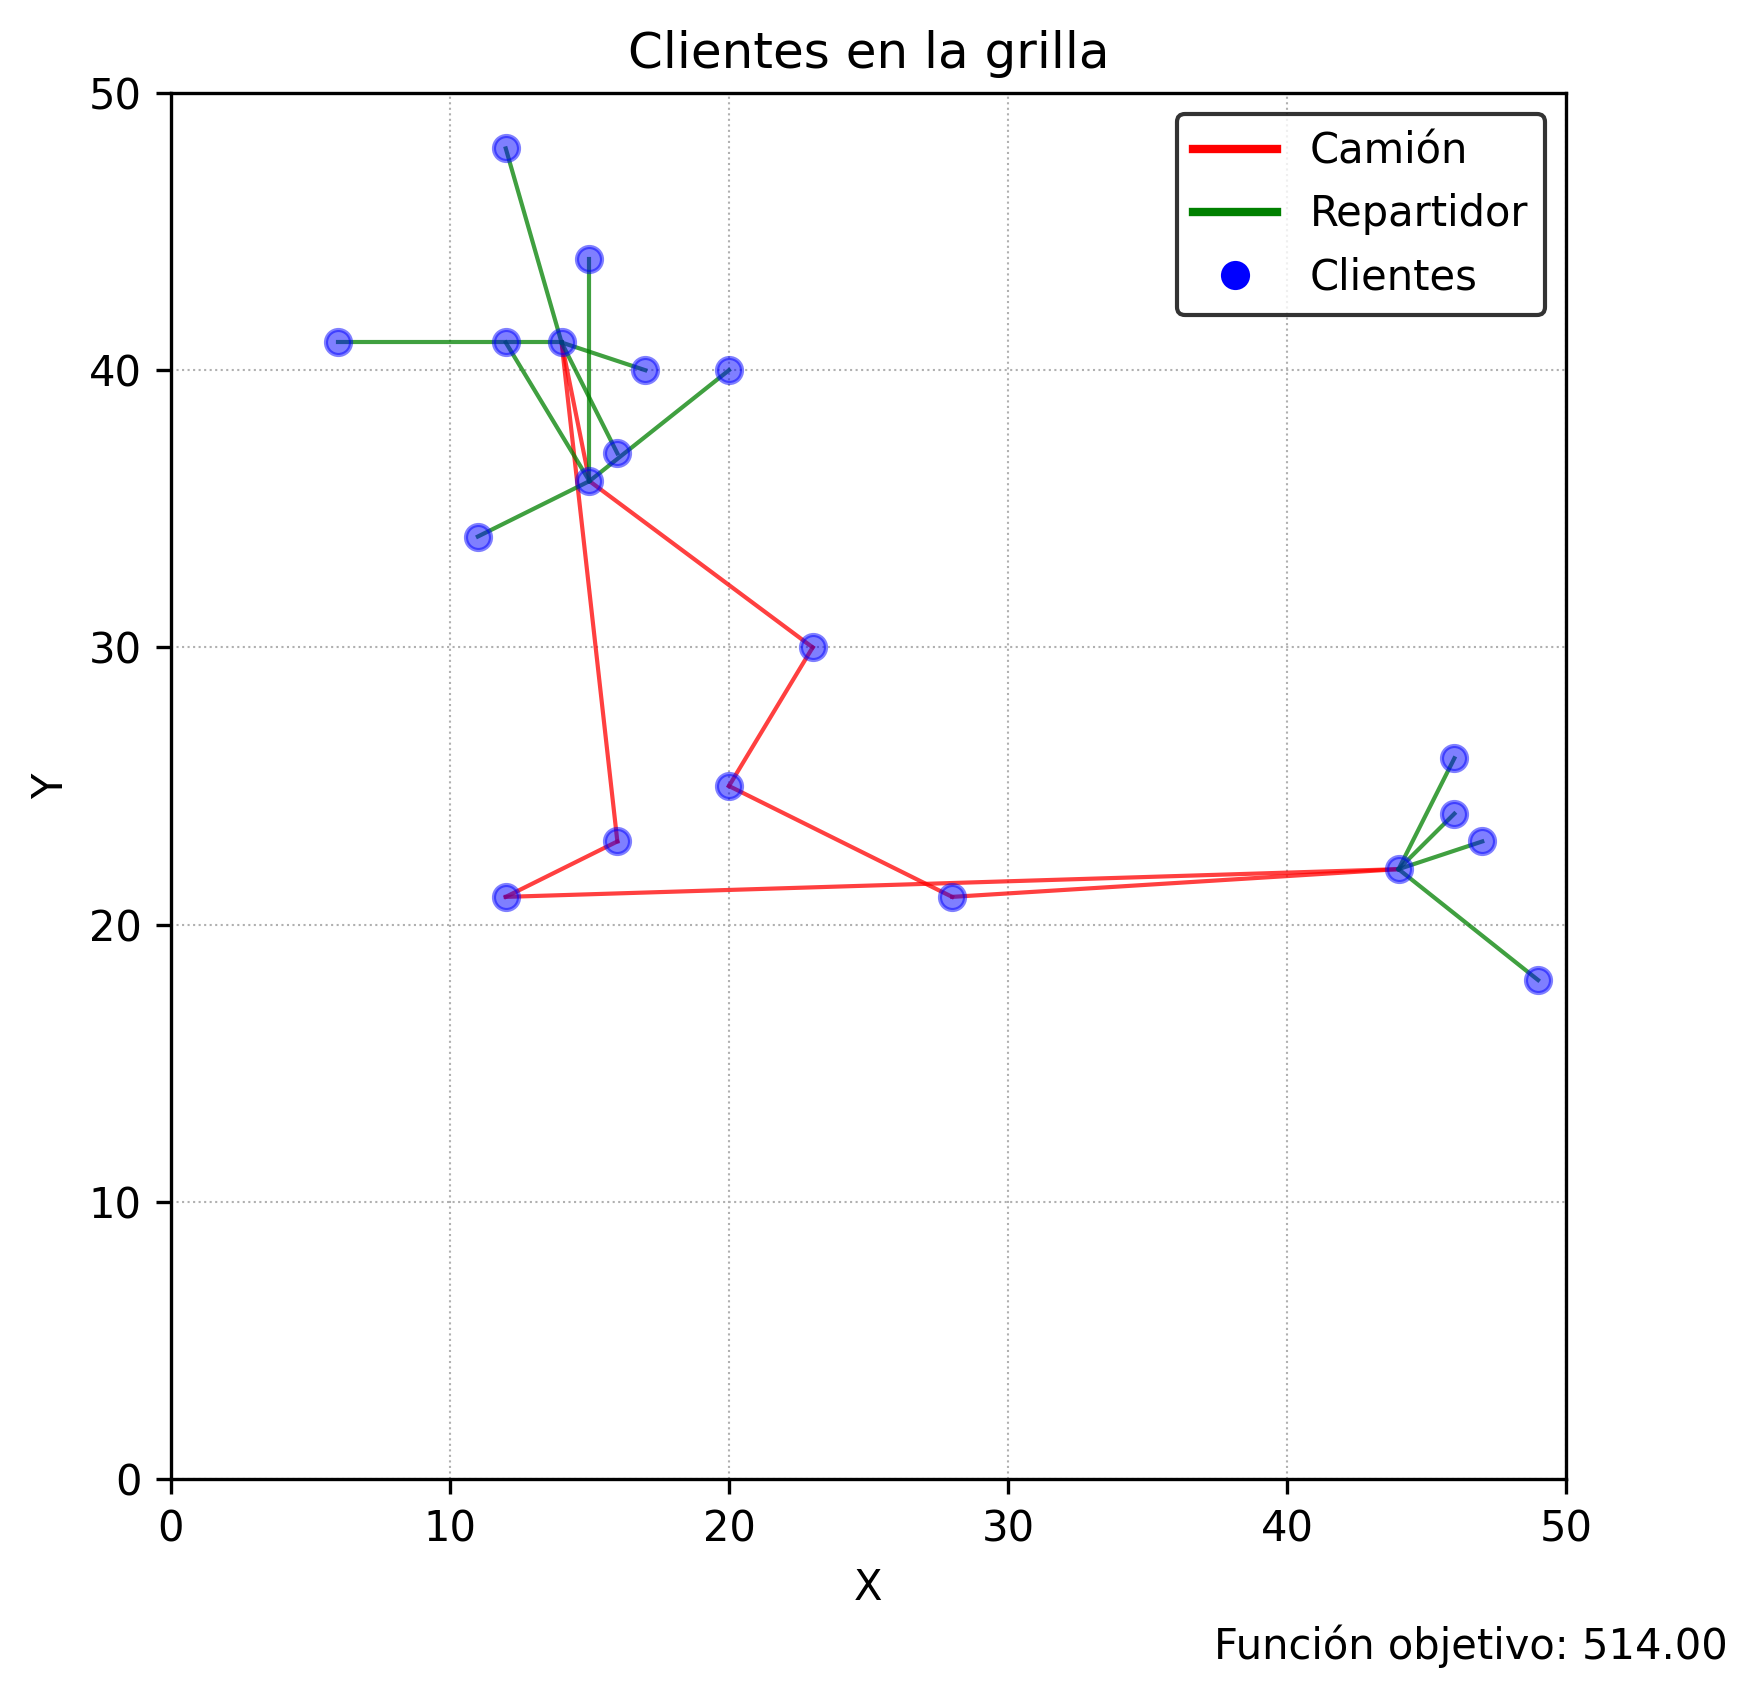
\includegraphics[width=\textwidth]{figuras/plano_clusters_cuatro_o_mas_0.png}
		\caption{Metodología con repartidores de al menos cuatro entregas (MR4)}
		\label{fig:sub3}
	\end{subfigure}
	\hfill
	\begin{subfigure}[b]{0.45\textwidth}
		\centering
		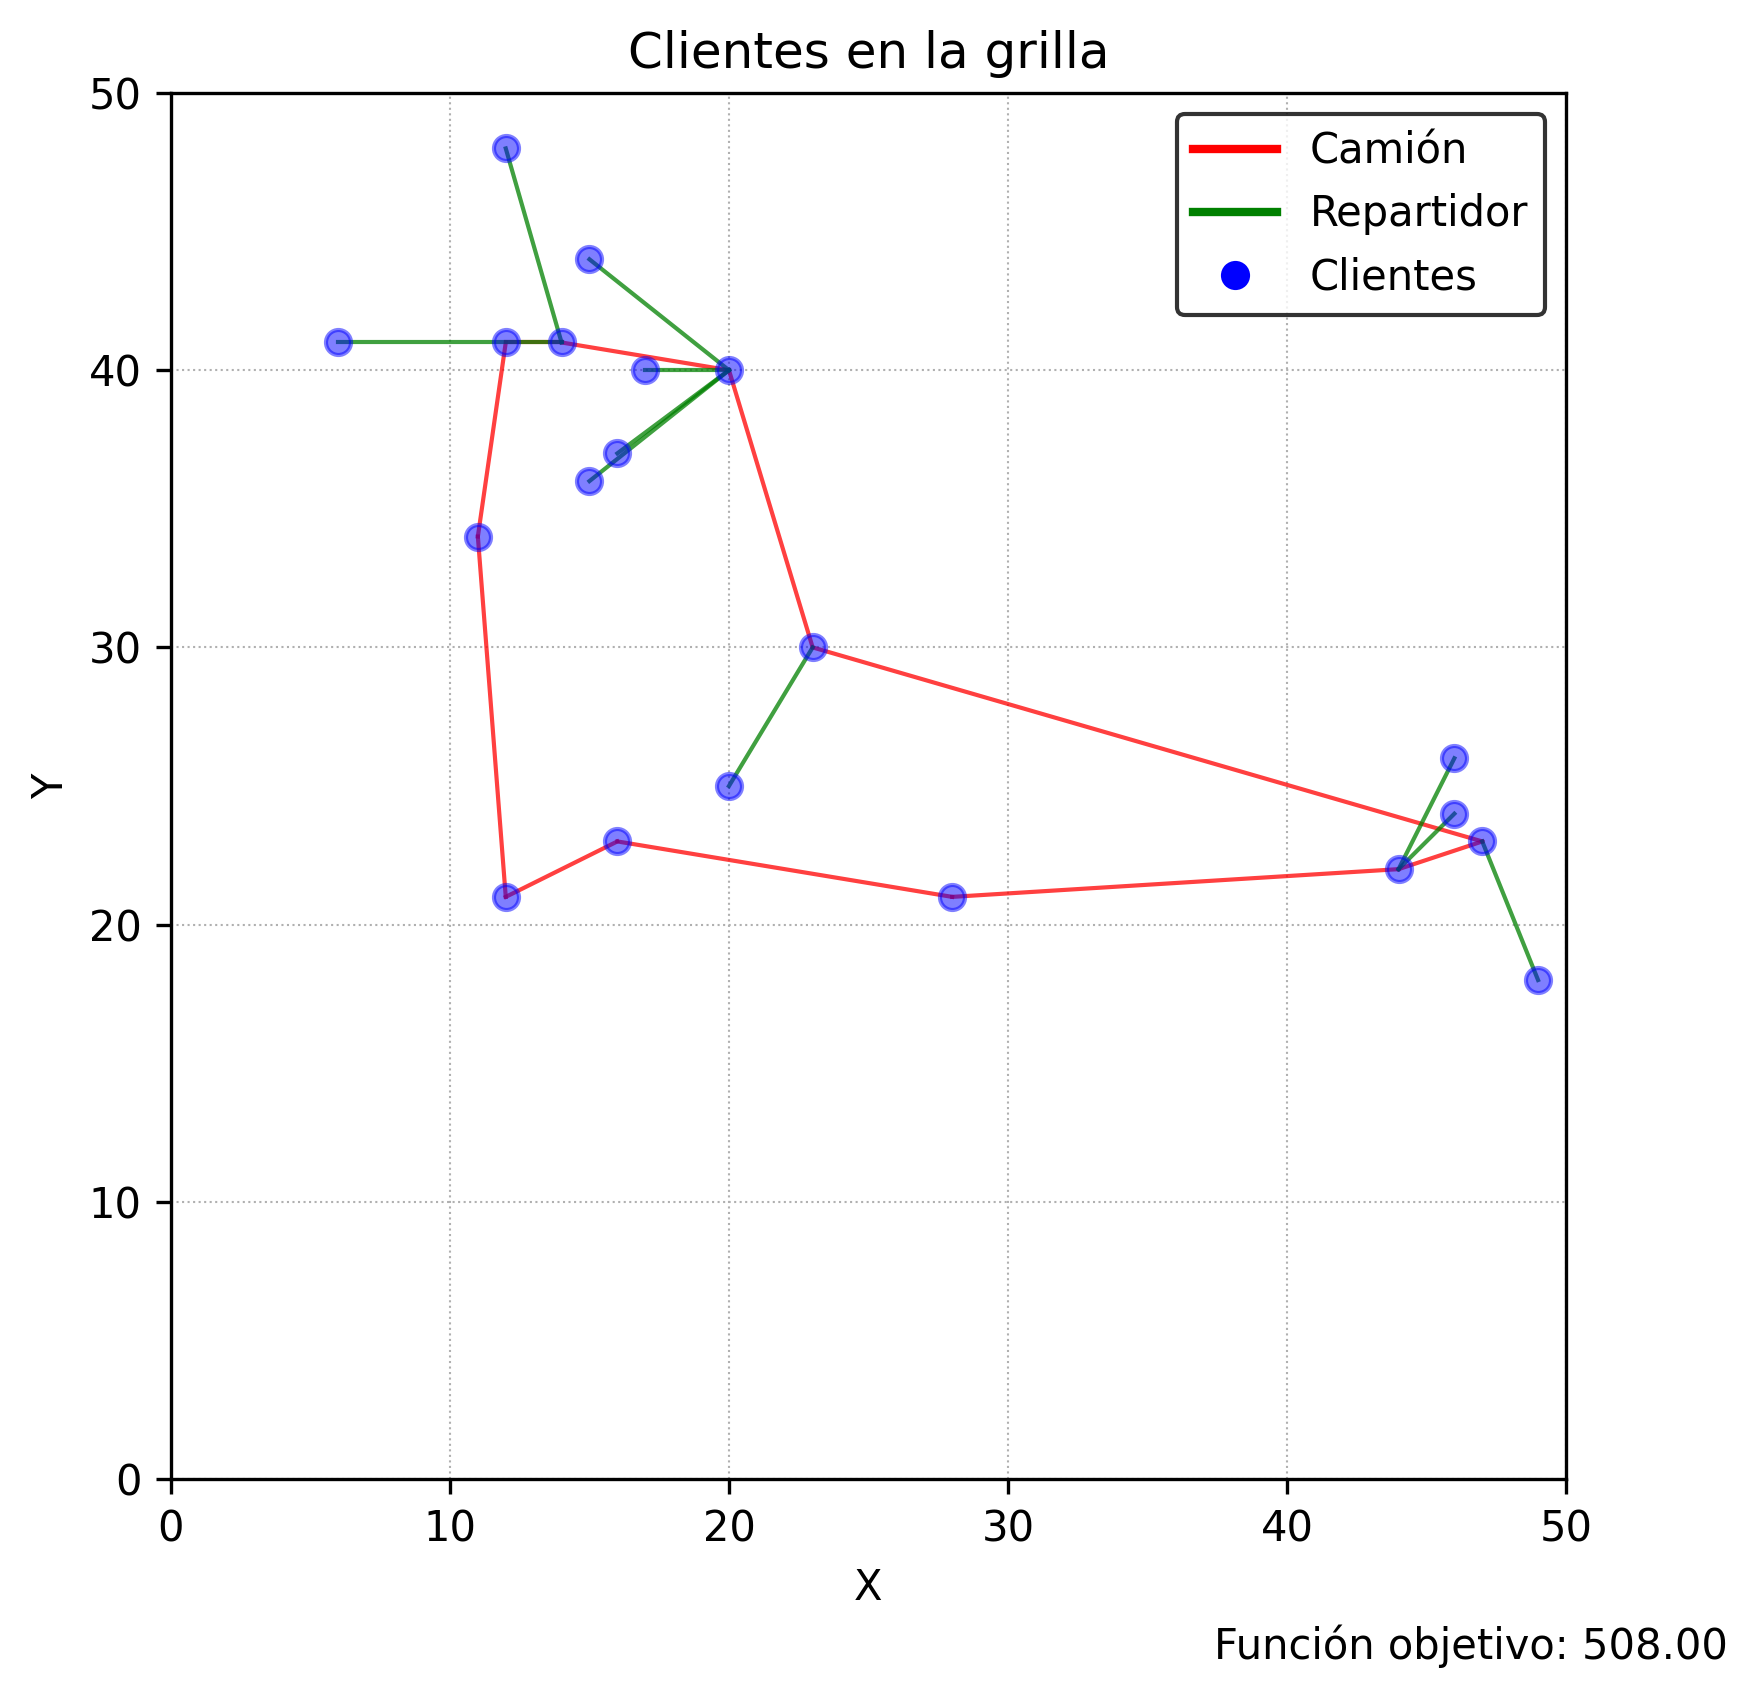
\includegraphics[width=\textwidth]{figuras/plano_clusters_exclusivos_0.png}
		\caption{Metodología con clientes exclusivos (MRE)}
		\label{fig:sub4}
	\end{subfigure}
	
	\caption{Optimización de una misma instancia de \textbf{clusters} con los distintos modelos.}
	\label{fig:compuesta2}
\end{figure}

\subsection{Análisis por metodología e instancia}
Con el objetivo de relevar diferencias en los costos logísticos, generamos dos tipos de instancias: 50 instancias con distribución uniforme y 32 instancias con estructura de tipo cluster. La cantidad de instancias del segundo tipo fue menor debido a que implicaron un tiempo de cómputo significativamente mayor, probablemente porque en estos casos las variables asociadas a los repartidores juegan un rol más determinante en la reducción de costos.

El criterio para la elección de los parámetros se basó en generar instancias con 20 clientes, buscando que fueran ejecutables en un tiempo razonable. Por otro lado, tanto el rango de movimiento como los costos asignados al repartidor y al camión fueron seleccionados de manera tal que permitieran un balance interesante entre ambas alternativas, favoreciendo como se esperaría en la realidad, el costo de los repartidores.
\clearpage

\begin{table}[htbp]
	\centering
	\begin{tabular}{ll}
		\hline
		\textbf{Parámetro} & \textbf{Valor} \\
		\hline
		Tamaño del grid & $50 \times 50$ \\
		Cantidad de clientes & 20 \\
		Rango del repartidor & 10 unidades \\
		Costo del repartidor (por unidad) & 2 \\
		Costo del camión (por unidad) & 5 \\
		Clientes refrigerados & 2 \\
		Clientes con entrega exclusiva & 5 \\
		\hline
	\end{tabular}
	\caption{Parámetros utilizados para la generación de instancias}
	\label{tab:parametros_instancias}
\end{table}


Todas las instancias, independientemente del tipo, fueron evaluadas utilizando los cuatro modelos propuestos. En la Figura~\ref{fig:comparacion_costos} se presentan los resultados obtenidos. Como era de esperarse, cualquier enfoque que incluya repartidores tiende a generar un menor costo total en comparación con el modelo TSP.

Tampoco resulta sorprendente que las instancias del tipo cluster presenten una mayor reducción de costos en comparación con las de distribución uniforme. Esto se debe a que, en estos casos, los recorridos entre clientes suelen ser más cortos y, además, facilita las condiciones para el uso de repartidores, lo que incrementa su impacto en la reducción del costo total.

Por otra parte, todas las instancias que los modelos MR4 y MRE, que incorporan restricciones adicionales respecto al modelo MR, presentan consistentemente un costo operativo mayor. Este resultado es coherente con lo esperado, dado que ambas metodologías derivan de MR, pero limitan el conjunto de soluciones.

\subsection{Conclusión}
Los resultados muestran que todas las metodologías propuestas permiten una reducción en el costo operativo de reparto en comparación con enfoques sin repartidores, tanto en instancias con clientes en una distribución uniforme como en aquellas con clusters.

En particular, la metodología con restricciones (MR) propuesta primero, resultó ser la de menor costo, alcanzando una mejora de hasta un -26,7\% en promedio frente a la metodología actual (TSP). En caso de tener que trabajar con alguna de las dos restricciones que eran deseables, se observó que la metodología con entregas exclusivas (MRE) presentó un impacto menor en el aumento de costos en comparación con MR4.

\begin{figure}[htbp]
	\centering
	
	\begin{subfigure}[b]{0.49\textwidth}
		\centering
		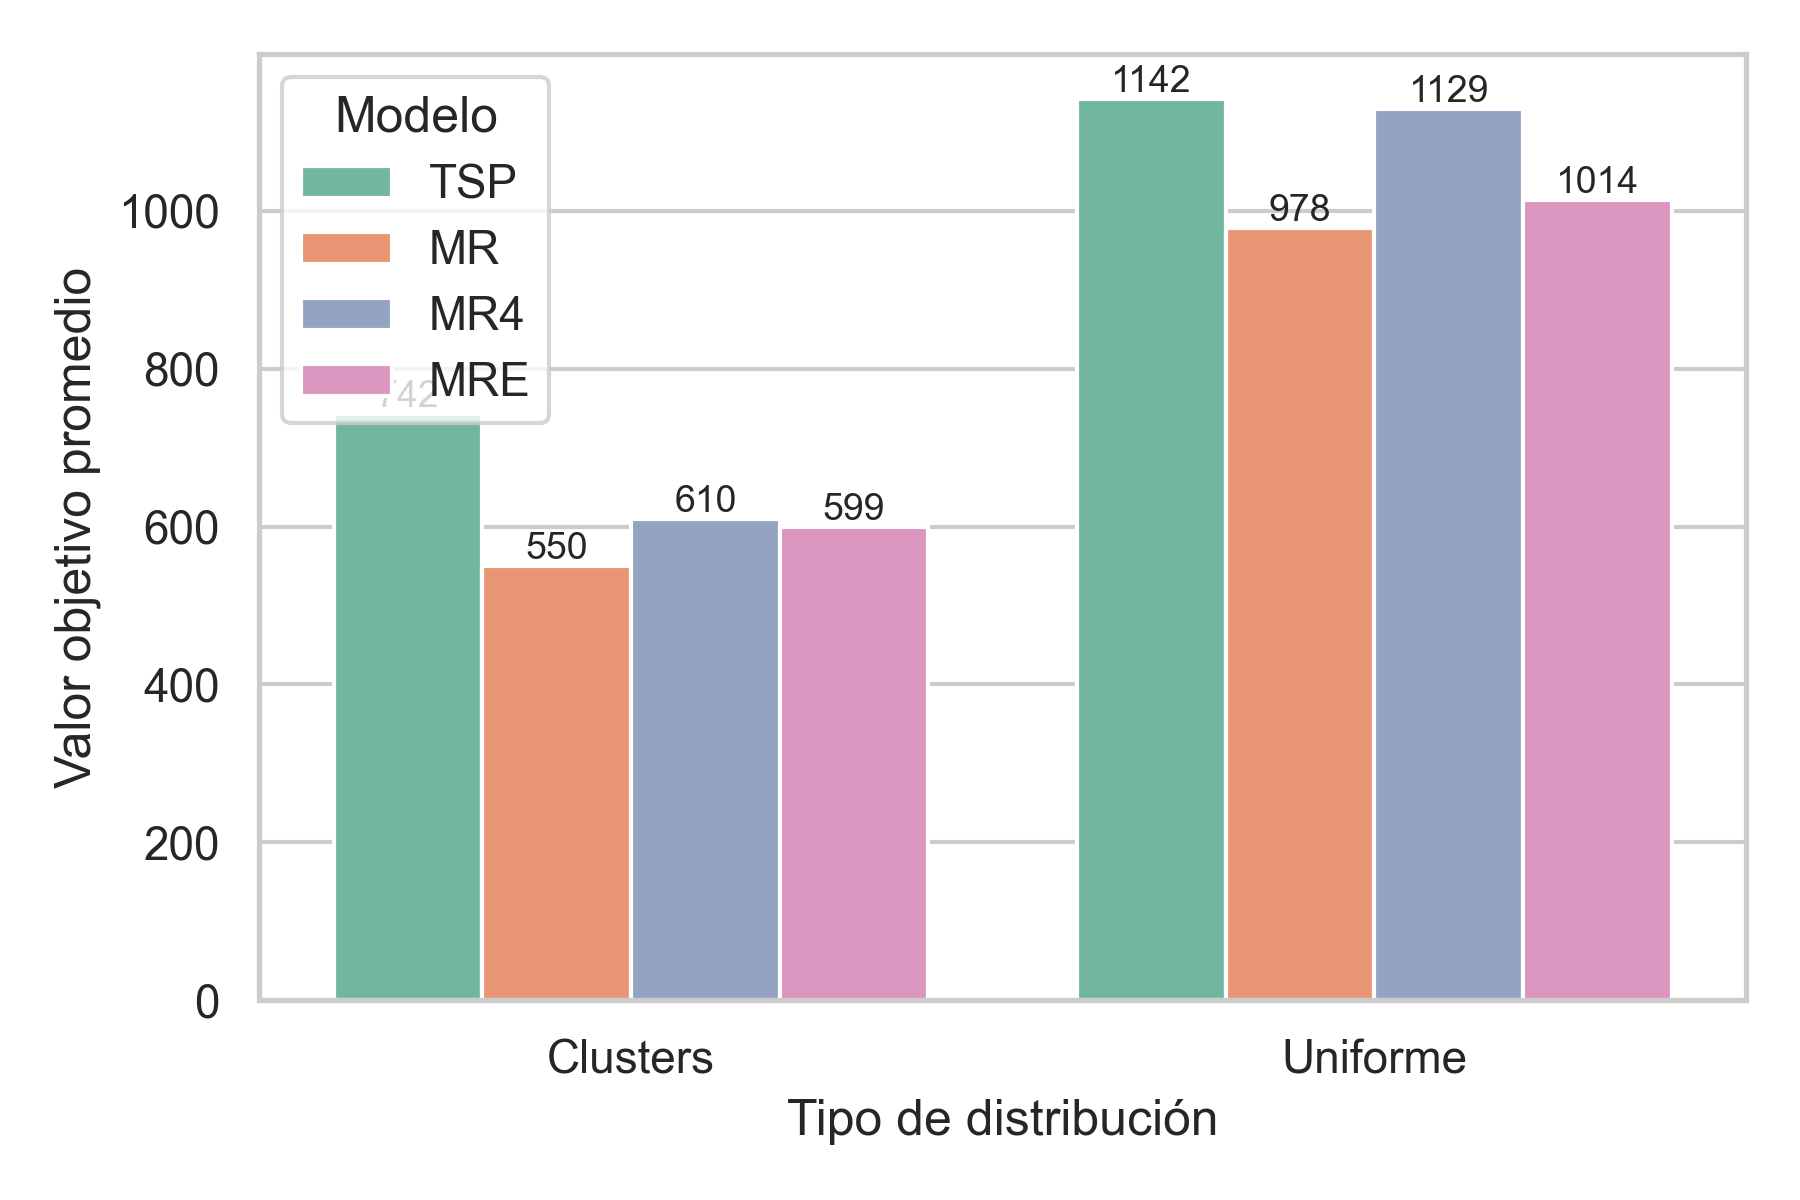
\includegraphics[width=\textwidth]{figuras/barras_costos.png}
		\caption{Valores objetivos promedio para cada tipo de distribución y metodología.}
		\label{fig:barras_costos}
	\end{subfigure}
	\hfill
	\begin{subfigure}[b]{0.49\textwidth}
		\centering
		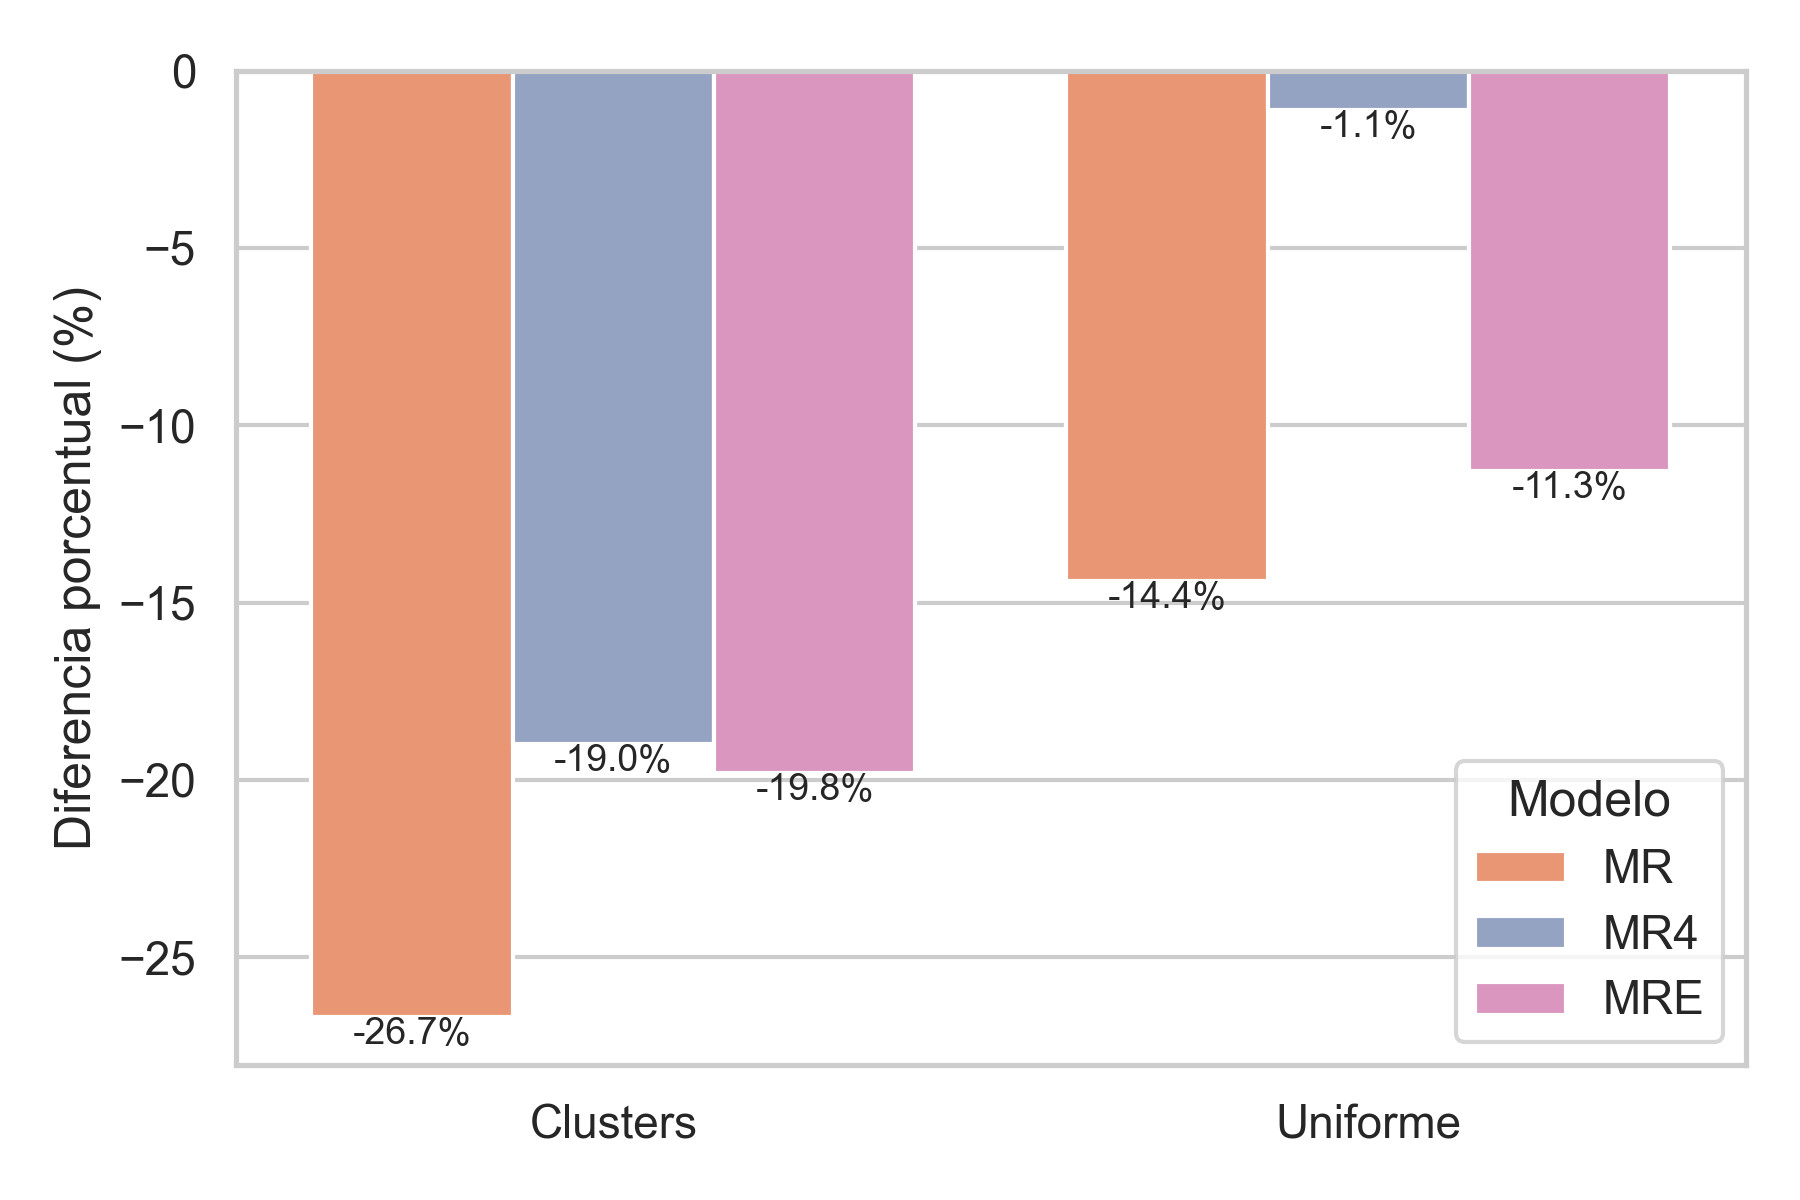
\includegraphics[width=\textwidth]{figuras/barras_diferencias_pct.png}
		\caption{Diferencia promedio de cada instancia con respecto al costo con TSP.}
		\label{fig:dif_pct_costos}
	\end{subfigure}
	
	\caption{Resultados agregados por metodología y tipo de distribución.}
	\label{fig:comparacion_costos}
\end{figure}


\clearpage

\section{Tiempos de cómputo CPLEX}

\end{document}
